\documentclass{article}\usepackage[]{graphicx}\usepackage[]{color}
%% maxwidth is the original width if it is less than linewidth
%% otherwise use linewidth (to make sure the graphics do not exceed the margin)
\makeatletter
\def\maxwidth{ %
  \ifdim\Gin@nat@width>\linewidth
    \linewidth
  \else
    \Gin@nat@width
  \fi
}
\makeatother

\definecolor{fgcolor}{rgb}{0.345, 0.345, 0.345}
\newcommand{\hlnum}[1]{\textcolor[rgb]{0.686,0.059,0.569}{#1}}%
\newcommand{\hlstr}[1]{\textcolor[rgb]{0.192,0.494,0.8}{#1}}%
\newcommand{\hlcom}[1]{\textcolor[rgb]{0.678,0.584,0.686}{\textit{#1}}}%
\newcommand{\hlopt}[1]{\textcolor[rgb]{0,0,0}{#1}}%
\newcommand{\hlstd}[1]{\textcolor[rgb]{0.345,0.345,0.345}{#1}}%
\newcommand{\hlkwa}[1]{\textcolor[rgb]{0.161,0.373,0.58}{\textbf{#1}}}%
\newcommand{\hlkwb}[1]{\textcolor[rgb]{0.69,0.353,0.396}{#1}}%
\newcommand{\hlkwc}[1]{\textcolor[rgb]{0.333,0.667,0.333}{#1}}%
\newcommand{\hlkwd}[1]{\textcolor[rgb]{0.737,0.353,0.396}{\textbf{#1}}}%

\usepackage{framed}
\makeatletter
\newenvironment{kframe}{%
 \def\at@end@of@kframe{}%
 \ifinner\ifhmode%
  \def\at@end@of@kframe{\end{minipage}}%
  \begin{minipage}{\columnwidth}%
 \fi\fi%
 \def\FrameCommand##1{\hskip\@totalleftmargin \hskip-\fboxsep
 \colorbox{shadecolor}{##1}\hskip-\fboxsep
     % There is no \\@totalrightmargin, so:
     \hskip-\linewidth \hskip-\@totalleftmargin \hskip\columnwidth}%
 \MakeFramed {\advance\hsize-\width
   \@totalleftmargin\z@ \linewidth\hsize
   \@setminipage}}%
 {\par\unskip\endMakeFramed%
 \at@end@of@kframe}
\makeatother

\definecolor{shadecolor}{rgb}{.97, .97, .97}
\definecolor{messagecolor}{rgb}{0, 0, 0}
\definecolor{warningcolor}{rgb}{1, 0, 1}
\definecolor{errorcolor}{rgb}{1, 0, 0}
\newenvironment{knitrout}{}{} % an empty environment to be redefined in TeX

\usepackage{alltt}

\usepackage{fancyhdr} % Required for custom headers
\usepackage{lastpage} % Required to determine the last page for the footer
\usepackage{extramarks} % Required for headers and footers
\usepackage{graphicx} % Required to insert images and make tiny font size
\usepackage{hyperref}
\usepackage{amsmath} %for binomial pdf
\usepackage{parskip} % so that there's space bw paragraphs
\usepackage{float}
\usepackage{amsfonts}

% Margins
\topmargin=-0.45in
\evensidemargin=0in
\oddsidemargin=0in
\textwidth=6.5in
\textheight=9.0in
\headsep=0.25in 

\linespread{1.1} % Line spacing

% Set up the header and footer
\pagestyle{fancy}
\lhead{STAT 532: Bayes} % Top left header
\chead{Midterm: Take Home} % Top center header
\rhead{Andrea Mack} % Top right header
\lfoot{10/17/2016} % Bottom left footer
\cfoot{} % Bottom center footer
\rfoot{Page\ \thepage\ of\ \pageref{LastPage}} % Bottom right footer
\renewcommand\headrulewidth{0.4pt} % Size of the header rule
\renewcommand\footrulewidth{0.4pt} % Size of the footer rule

\setlength\parindent{0pt} % Removes all indentation from paragraphs
\setlength\parskip{0.5cm}
\restylefloat{table}

%----------------------------------------------------------------------------------------
%	DOCUMENT STRUCTURE COMMANDS
%	Skip this unless you know what you're doing
%----------------------------------------------------------------------------------------

% Header and footer for when a page split occurs within a problem environment
\newcommand{\enterProblemHeader}[1]{
\nobreak\extramarks{#1}{#1 continued on next page\ldots}\nobreak
\nobreak\extramarks{#1 (continued)}{#1 continued on next page\ldots}\nobreak
}

% Header and footer for when a page split occurs between problem environments
\newcommand{\exitProblemHeader}[1]{
\nobreak\extramarks{#1 (continued)}{#1 continued on next page\ldots}\nobreak
\nobreak\extramarks{#1}{}\nobreak
}


%----------------------------------------------------------------------------------------%
\IfFileExists{upquote.sty}{\usepackage{upquote}}{}
\begin{document}


\begin{enumerate}
\addtocounter{enumi}{1}
\item%2 

\begin{enumerate}
\item%2a
The Poisson model is reasonable because the number of bikes represents finite count data and each hub can  be considered an enclosed space. 

Let $\underset{\sim}{y} \sim$ POISSON($\theta$),

Then $\theta$ represents the true average number of bikes per hub and each $y_{i}$ represents the count of bikes at the ith hub, which each are assumed to come from the same distribution, with the same mean ($\theta$).

\item%2b
The Gamma distribution is often chosen as a prior on a POISSON parameter. The POISSON parameter represents the mean as well as the variation in the bike counts. Since variances are always positive, and the family of Gamma distributions have a support of (0,infinite), it is a reasonable choice. While choosing a member of the Gamma distributions on $\theta$ is convenient because it serves as a conjugate prior, that is not the justification I am using. It is, however, a nice property.

$\alpha$ can be thought of as the prior count and $\beta$ can be thought of as the prior number of observations. I do not have any prior knowledge, so I will set the prior number of observations to 1, and make the distribution improper by choosing the prior number of counts as 0. Doing so makes the prior distribution flat, as also can be seen in the first two moments.

\item%2c

$p(\theta | \underset{\sim}{y}) \sim$ GAMMA($\Sigma y_{i} + \alpha, n + \beta$)

when $y_{i} \sim$ POISSON($\theta$) and

$\theta \sim$ GAMMA($\alpha,\beta$).

p($\theta | \underset{\sim}{y}) \propto \int_{\theta} p(\underset{\sim}{y} | \theta) \times p(\theta$) d$\theta$

$\propto \int_{\theta}$ $\frac{\theta^{\Sigma y_{i}}e^{-n\theta}}{\Pi y_{i}!} \times \frac{\beta^{\alpha}\theta^{\alpha - 1}e^{-\theta\beta}}{\Gamma(\alpha)} d\theta$

$\propto \int_{\theta}$ $\frac{\theta^{\Sigma y_{i} + \alpha - 1}e^{-\theta(n+\beta)}\beta^{\alpha}}{\Pi y_{i}\Gamma(\alpha)} d\theta$

$\propto$ GAMMA($\Sigma y_{i} + \alpha$, $n+\beta$)

$\propto$ GAMMA(9435 + 0, 392 + 1)

$\propto$ GAMMA(9435, 393)



\item%2d
p($y^{*} | \underset{\sim}{y})$ = $\int_{\theta} p(\Sigma y^{*} | \theta) \times p(\theta | \underset{\sim}{y}) d\theta$

From the notes, p($y^{*} | \underset{\sim}{y}) \sim$ NEGBINOM($\Sigma y_{i} + \alpha, n + \beta$)

But rather than drawing samples from the Negative Binomial model, we can use the MC algorithm to draw predictions using random draws from the posterior of $\theta$ and the conditional, $y^{*} | \theta \sim$ POISSON($\theta$).

The posterior predicted values generated are plotted below. There is much less variation in the posterior of $\theta$ than in the posterior predictions. Since we are using two draws for each prediction (one from the posterior on $\theta$ and one from the predictive on $y^{*}$), it makes sense that there should be more variation in the $y^{*}$ predictive distribution. Both have a fairly symmetrical shape and nearly the same center. I am surprised with the degree of accuracy shown in the posterior of $\theta$ compared to the predictions of $y^{*}$.
\begin{knitrout}
\definecolor{shadecolor}{rgb}{0.969, 0.969, 0.969}\color{fgcolor}

{\centering 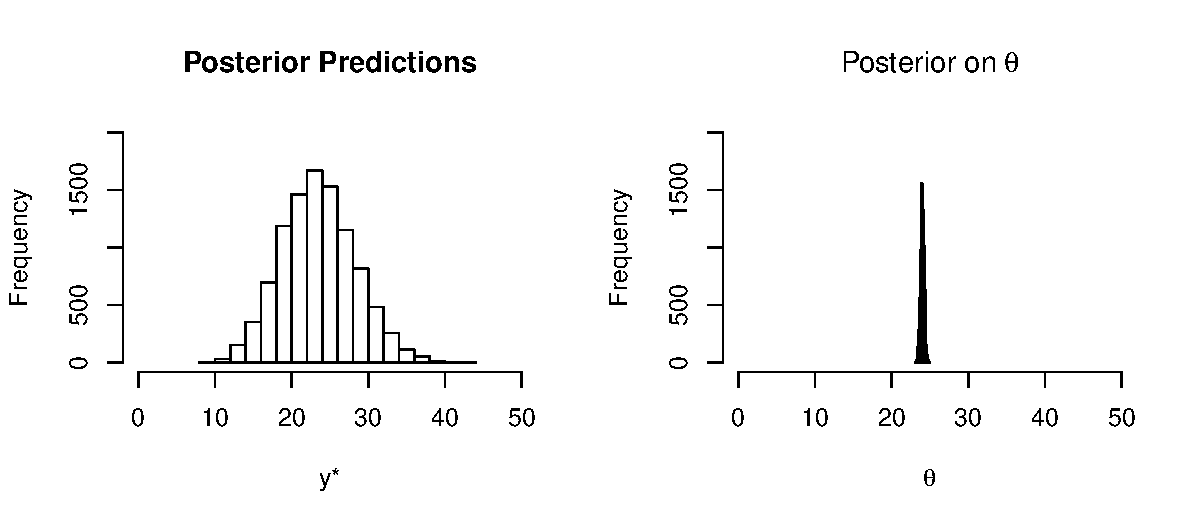
\includegraphics[width=\maxwidth]{figure/prob2d-1} 

}



\end{knitrout}

\item %2e


The 95\% credible interval is estimated to be (2.9407029, 3.061808) bikes per slot and the point estimate is 3.00102 bikes per slot.

\item %2f


The MAP point estimate is within the interval (24.18,24.19] while the mean of the posterior distribution should theoretically be 24.0076336 and the mean based on the simulations was 24.0081603. Bother are less than the MAP point estimate. No the mean is not the MAP point estimate. 

\item %2g


The estimated highest 95\% posterior density region is (23.33, 24.65] compared to the 95\% credible interval of (23.5256232, 24.4944641). My bins were 0.01 units in estimating the HPD region.

My HPD region is slightly wider than the credible interval and was estimated as the 94.96\% HPD region. It is likely the differences are due to the size of my bins so yes, I would say the 95\% HPD region is the 95\% credible interval here.

\end{enumerate}

\item%3
\begin{enumerate}
\item%3a


I do not have any prior information. So I will choose a weakly informative prior, and use the same one for both sets of years, as I do not have any more information about one year over the other.

The prior mean for both sets of years will be set to 0 and the prior variance for both sets of years will be set to 100. The prior variance is set to this based on the empirical rule, we expect about 95\% of the data to lie within 2sd's of the mean. I'll say I expect to be within about 20 dollars of the true mean.

I will generalize with $\theta$ and $\sigma^2$ since I am assuming the same prior for both time periods.

$\theta \sim$ N(0, 100)

Where $\nu_{o}$ represents the prior number of observations and $\sigma^2_{o}$ represents the prior sample variance, I will set these to 1 and 100 respectively, using 100 with the same idea as above in mind.

$\sigma^2 \sim$ INVGAM(0.5,50)

$\implies \frac{1}{\sigma^2} \sim$ INVGAM(0.5,50)}

\item%3b

Below are plots to assess the covergence of the joint posterior as well as the marginals for both sets of years.

Both joint posteriors appear to converge within the first few iterations.

\begin{knitrout}
\definecolor{shadecolor}{rgb}{0.969, 0.969, 0.969}\color{fgcolor}

{\centering 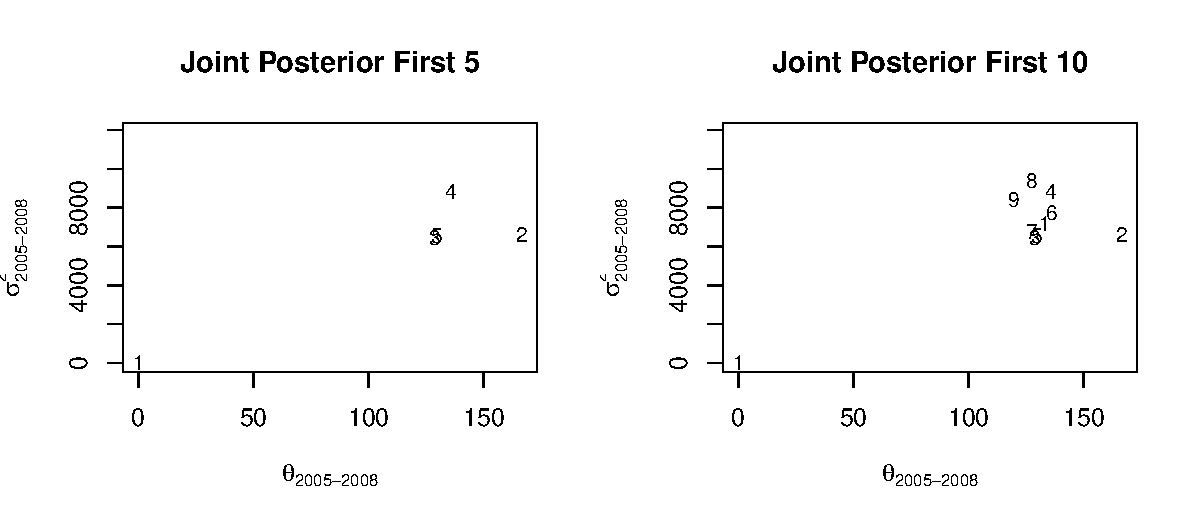
\includegraphics[width=\maxwidth]{figure/prob3b-1} 

}




{\centering 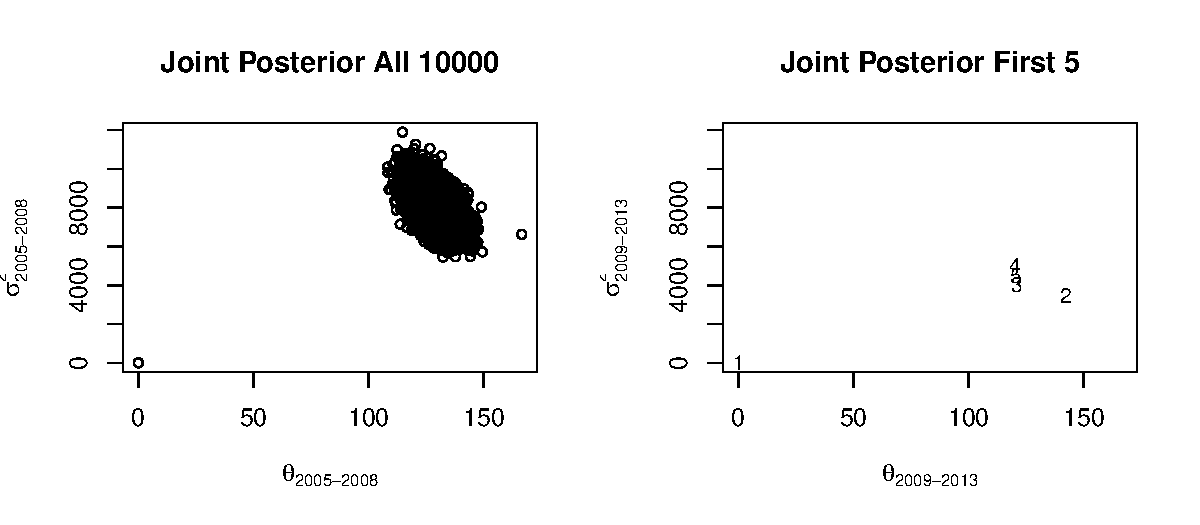
\includegraphics[width=\maxwidth]{figure/prob3b-2} 

}




{\centering 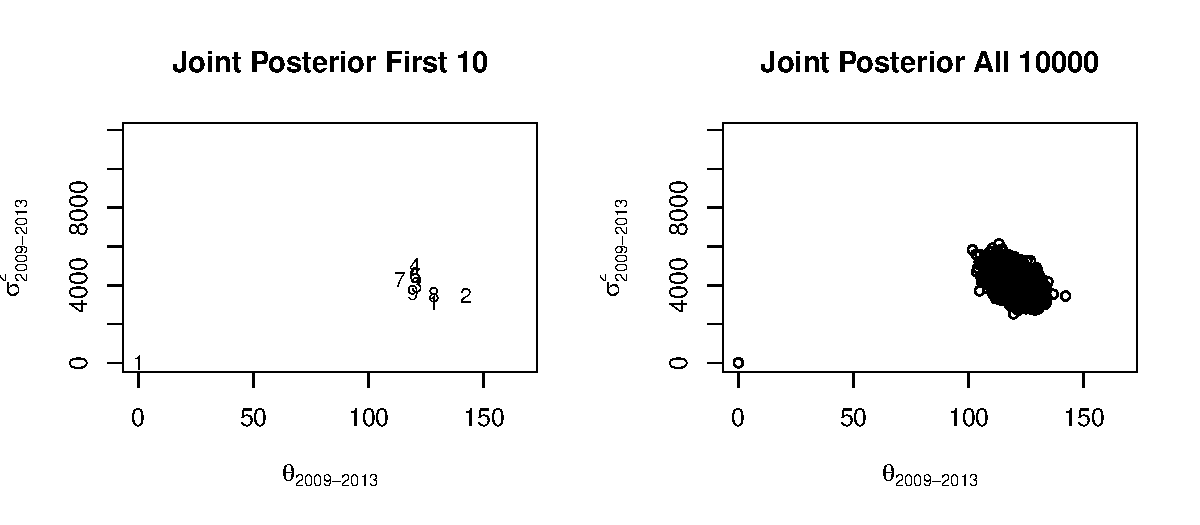
\includegraphics[width=\maxwidth]{figure/prob3b-3} 

}




{\centering 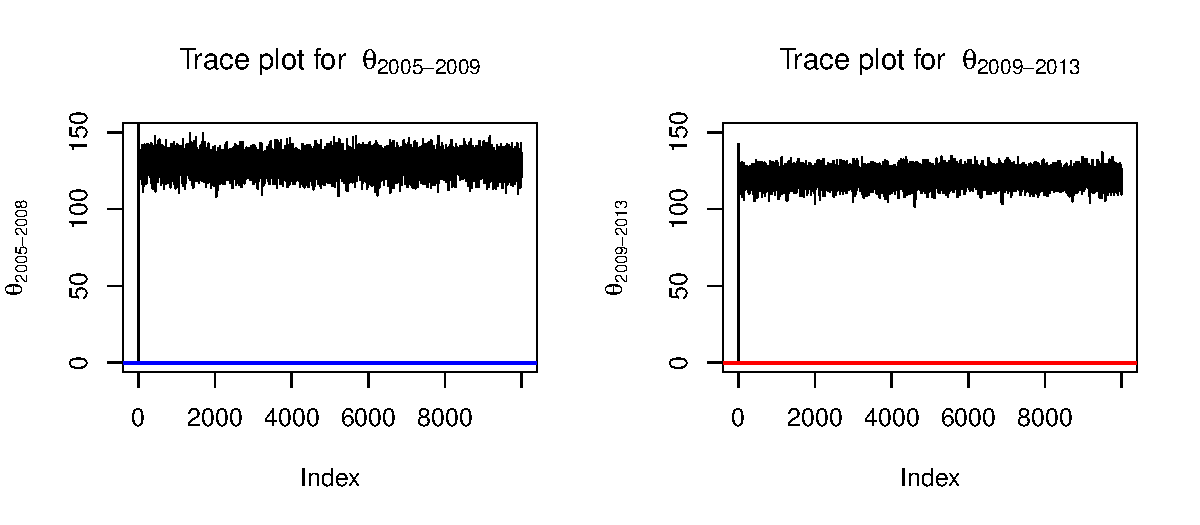
\includegraphics[width=\maxwidth]{figure/prob3b-4} 

}




{\centering 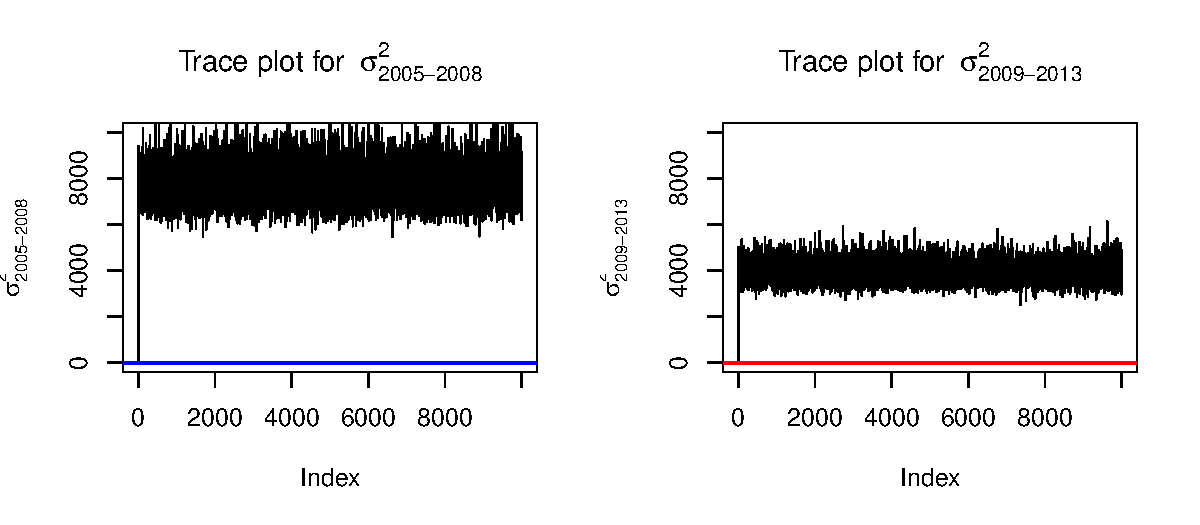
\includegraphics[width=\maxwidth]{figure/prob3b-5} 

}



\end{knitrout}
\newpage

\item %3c
Below are the marginal posteriors of the $\theta$s.

\begin{knitrout}
\definecolor{shadecolor}{rgb}{0.969, 0.969, 0.969}\color{fgcolor}

{\centering 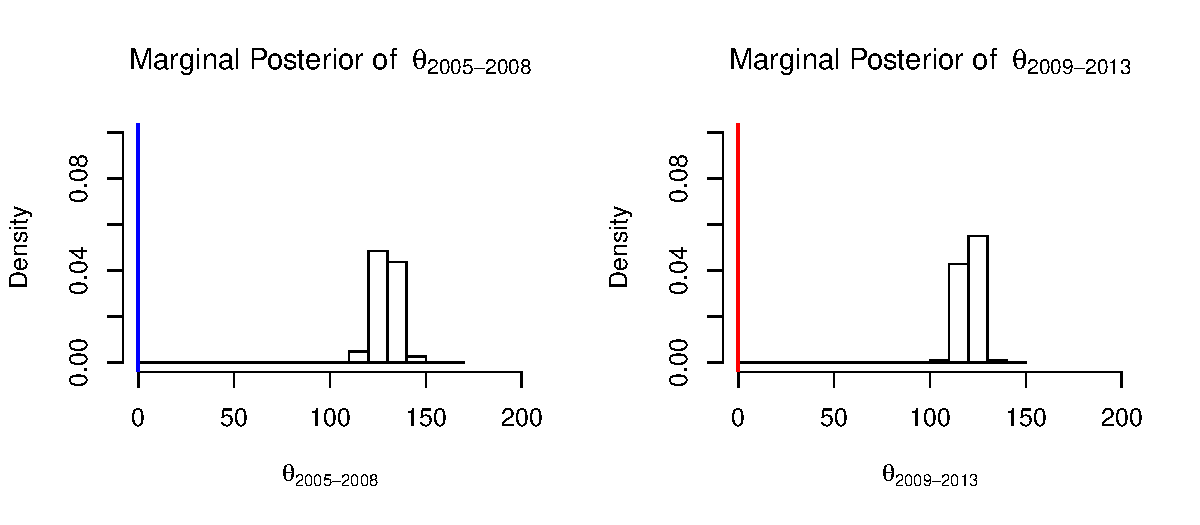
\includegraphics[width=\maxwidth]{figure/prob3c-1} 

}



\end{knitrout}

\item%3d


Where c = \$10/$ft^{2}$, the Pr($|\theta_{2} - \theta_{1}| > c$) is estimated to be 0.2196 using the GIBBs algorithm.

\item %3e
In part (d) I found that 21.96\% of the iterations were more than \$10/$ft^{2}$ apart. Since this is a Bayesian framework, we would say there is a 21.96\% that a change point has occured. 

The observed difference in simulated posterior means was 8.7649131 with added individual variances of 54.0511367, making the standard deviation around 7. Note, we can only do this if we assume the two time periods are independent, which they surely are not, and a covariance term could increase or decrease this and with the variable housing markets, I'm not sure which would be more accurate. Considering the size of the observed difference, there is quite a bit of uncertainty. But I think relative to all of this information, the interpretation of the probability of a point change is representative of the uncertainty and the difference in means.
\end{enumerate}
\end{enumerate}

\appendix
\section*{R Code}
{\tiny
\begin{knitrout}
\definecolor{shadecolor}{rgb}{0.969, 0.969, 0.969}\color{fgcolor}\begin{kframe}
\begin{alltt}
\hlkwd{require}\hlstd{(xtable)}
\hlkwd{require}\hlstd{(ggplot2)}
\hlkwd{require}\hlstd{(dplyr)} \hlcom{#between()}
\hlkwd{require}\hlstd{(truncnorm)} \hlcom{#work with truncated norm}
\hlkwd{require}\hlstd{(LearnBayes)}
\hlstd{opts_chunk}\hlopt{$}\hlkwd{set}\hlstd{(}\hlkwc{echo} \hlstd{=} \hlnum{FALSE}\hlstd{,} \hlkwc{warning} \hlstd{=} \hlnum{FALSE}\hlstd{,} \hlkwc{fig.align} \hlstd{=} \hlstr{'center'}\hlstd{,} \hlkwc{fig.height} \hlstd{=} \hlnum{3.5}\hlstd{,} \hlkwc{fig.width} \hlstd{=} \hlnum{4}\hlstd{)}
\end{alltt}
\end{kframe}
\end{knitrout}
\begin{knitrout}
\definecolor{shadecolor}{rgb}{0.969, 0.969, 0.969}\color{fgcolor}\begin{kframe}
\begin{alltt}
\hlstd{bikes} \hlkwb{<-} \hlkwd{read.csv}\hlstd{(}\hlstr{"MidtermBikes.csv"}\hlstd{)}
\hlkwd{head}\hlstd{(bikes)}
\end{alltt}
\end{kframe}
\end{knitrout}
\begin{enumerate}

\setcounter{enumi}{2}
\item%2
\setcounter{enumi}{3}
\begin{enumerate}
\item%2c
\begin{knitrout}
\definecolor{shadecolor}{rgb}{0.969, 0.969, 0.969}\color{fgcolor}\begin{kframe}
\begin{alltt}
\hlstd{yi} \hlkwb{<-} \hlstd{bikes}\hlopt{$}\hlstd{bikes.rented}
\hlstd{sum.yi} \hlkwb{<-} \hlkwd{sum}\hlstd{(yi)}
\hlstd{n.yi} \hlkwb{<-} \hlkwd{length}\hlstd{(yi)}

\hlstd{alpha} \hlkwb{=} \hlnum{0}
\hlstd{beta} \hlkwb{=} \hlnum{1}
\end{alltt}
\end{kframe}
\end{knitrout}
\begin{knitrout}
\definecolor{shadecolor}{rgb}{0.969, 0.969, 0.969}\color{fgcolor}\begin{kframe}
\begin{alltt}
\hlcom{#posterior on theta}
\hlkwd{set.seed}\hlstd{(}\hlnum{532}\hlstd{)}
\hlstd{theta_i} \hlkwb{<-} \hlkwd{rgamma}\hlstd{(}\hlnum{10000}\hlstd{, alpha} \hlopt{+} \hlstd{sum.yi, beta} \hlopt{+} \hlstd{n.yi)}
\end{alltt}
\end{kframe}
\end{knitrout}
\item%2d
\begin{knitrout}
\definecolor{shadecolor}{rgb}{0.969, 0.969, 0.969}\color{fgcolor}\begin{kframe}
\begin{alltt}
\hlcom{#posterior predictive}
\hlstd{ystar} \hlkwb{<-} \hlkwd{c}\hlstd{(}\hlkwd{rep}\hlstd{(}\hlnum{0}\hlstd{,}\hlnum{10000}\hlstd{))}

\hlkwa{for}\hlstd{(i} \hlkwa{in} \hlnum{1}\hlopt{:}\hlnum{10000}\hlstd{)\{}
\hlstd{ystar[i]} \hlkwb{<-} \hlkwd{rpois}\hlstd{(}\hlnum{1}\hlstd{, theta_i[i])}
\hlstd{\}}

\hlkwd{par}\hlstd{(}\hlkwc{mfrow}\hlstd{=}\hlkwd{c}\hlstd{(}\hlnum{1}\hlstd{,}\hlnum{2}\hlstd{))}
\hlkwd{hist}\hlstd{(ystar,} \hlkwc{main} \hlstd{=} \hlstr{"Posterior Predictions"}\hlstd{,} \hlkwc{xlab} \hlstd{=}
       \hlstr{"y*"}\hlstd{,} \hlkwc{xlim}\hlstd{=}\hlkwd{c}\hlstd{(}\hlnum{0}\hlstd{,}\hlnum{50}\hlstd{),} \hlkwc{ylim} \hlstd{=} \hlkwd{c}\hlstd{(}\hlnum{0}\hlstd{,}\hlnum{2000}\hlstd{))}
\hlkwd{hist}\hlstd{(theta_i,} \hlkwc{main} \hlstd{=} \hlkwd{expression}\hlstd{(}\hlstr{"Posterior on"} \hlopt{~} \hlstd{theta),}
     \hlkwc{xlab} \hlstd{=} \hlkwd{expression}\hlstd{(theta),} \hlkwc{xlim}\hlstd{=}\hlkwd{c}\hlstd{(}\hlnum{0}\hlstd{,}\hlnum{50}\hlstd{),} \hlkwc{ylim} \hlstd{=} \hlkwd{c}\hlstd{(}\hlnum{0}\hlstd{,}\hlnum{2000}\hlstd{))}
\end{alltt}
\end{kframe}
\end{knitrout}
\item%2e
\begin{knitrout}
\definecolor{shadecolor}{rgb}{0.969, 0.969, 0.969}\color{fgcolor}\begin{kframe}
\begin{alltt}
\hlstd{lb} \hlkwb{<-} \hlkwd{qgamma}\hlstd{(}\hlnum{0.025}\hlstd{,} \hlkwc{shape} \hlstd{= alpha} \hlopt{+} \hlstd{sum.yi,} \hlkwc{rate} \hlstd{= beta} \hlopt{+} \hlstd{n.yi)}

\hlstd{ub} \hlkwb{<-} \hlkwd{qgamma}\hlstd{(}\hlnum{0.975}\hlstd{,} \hlkwc{shape} \hlstd{= alpha} \hlopt{+} \hlstd{sum.yi,} \hlkwc{rate} \hlstd{= beta} \hlopt{+} \hlstd{n.yi)}

\hlstd{point.est} \hlkwb{<-} \hlkwd{mean}\hlstd{(theta_i)}\hlopt{/}\hlnum{8}
\end{alltt}
\end{kframe}
\end{knitrout}
\item%2f
\begin{knitrout}
\definecolor{shadecolor}{rgb}{0.969, 0.969, 0.969}\color{fgcolor}\begin{kframe}
\begin{alltt}
\hlstd{theta_i.binned} \hlkwb{<-} \hlkwd{cut}\hlstd{(theta_i,} \hlkwc{breaks} \hlstd{=} \hlkwd{c}\hlstd{(}\hlkwd{seq}\hlstd{(}\hlkwd{range}\hlstd{(theta_i)[}\hlnum{1}\hlstd{]}\hlopt{-}\hlnum{0.01}\hlstd{,}\hlkwd{range}\hlstd{(theta_i)[}\hlnum{2}\hlstd{]}\hlopt{+}\hlnum{0.01}\hlstd{,} \hlkwc{by} \hlstd{=} \hlnum{0.01}\hlstd{)))}
\hlstd{map.theta_i} \hlkwb{<-} \hlstd{theta_i.binned[}\hlkwd{max}\hlstd{(}\hlkwd{tabulate}\hlstd{(theta_i.binned))]}
\hlstd{mean.theta_i.sim} \hlkwb{<-} \hlkwd{mean}\hlstd{(theta_i)}
\hlstd{mean.theta_i.theoretical} \hlkwb{<-} \hlstd{(alpha} \hlopt{+} \hlstd{sum.yi)}\hlopt{/}\hlstd{(n.yi}\hlopt{+}\hlstd{beta)}
\end{alltt}
\end{kframe}
\end{knitrout}
\item%2g
\begin{knitrout}
\definecolor{shadecolor}{rgb}{0.969, 0.969, 0.969}\color{fgcolor}\begin{kframe}
\begin{alltt}
\hlstd{it} \hlkwb{<-} \hlkwd{table}\hlstd{(theta_i.binned)}

\hlstd{it1} \hlkwb{<-} \hlstd{it} \hlopt{-} \hlnum{1}

\hlstd{pd1} \hlkwb{<-} \hlstd{(}\hlkwd{sum}\hlstd{(it1[it1}\hlopt{>=}\hlnum{0}\hlstd{])} \hlopt{-} \hlkwd{sum}\hlstd{(it1))}\hlopt{/}\hlkwd{length}\hlstd{(theta_i)}

\hlstd{it2} \hlkwb{<-} \hlstd{it} \hlopt{-} \hlnum{2}

\hlstd{pd2} \hlkwb{<-} \hlstd{(}\hlkwd{sum}\hlstd{(it2[it2}\hlopt{>=}\hlnum{0}\hlstd{])} \hlopt{-} \hlkwd{sum}\hlstd{(it2))}\hlopt{/}\hlkwd{length}\hlstd{(theta_i)}

\hlstd{it3} \hlkwb{<-} \hlstd{it} \hlopt{-} \hlnum{3}

\hlstd{pd3} \hlkwb{<-} \hlstd{(}\hlkwd{sum}\hlstd{(it3[it3}\hlopt{>=}\hlnum{0}\hlstd{])} \hlopt{-} \hlkwd{sum}\hlstd{(it3))}\hlopt{/}\hlkwd{length}\hlstd{(theta_i)}

\hlstd{it5} \hlkwb{<-} \hlstd{it} \hlopt{-} \hlnum{5}

\hlstd{pd5} \hlkwb{<-} \hlstd{(}\hlkwd{sum}\hlstd{(it5[it5}\hlopt{>=}\hlnum{0}\hlstd{])} \hlopt{-} \hlkwd{sum}\hlstd{(it5))}\hlopt{/}\hlkwd{length}\hlstd{(theta_i)}

\hlstd{it8} \hlkwb{<-} \hlstd{it} \hlopt{-} \hlnum{8}

\hlstd{pd8} \hlkwb{<-} \hlstd{(}\hlkwd{sum}\hlstd{(it8[it8}\hlopt{>=}\hlnum{0}\hlstd{])} \hlopt{-} \hlkwd{sum}\hlstd{(it8))}\hlopt{/}\hlkwd{length}\hlstd{(theta_i)}

\hlstd{it7} \hlkwb{<-} \hlstd{it} \hlopt{-} \hlnum{7}

\hlstd{pd7} \hlkwb{<-} \hlstd{(}\hlkwd{sum}\hlstd{(it7[it7}\hlopt{>=}\hlnum{0}\hlstd{])} \hlopt{-} \hlkwd{sum}\hlstd{(it7))}\hlopt{/}\hlkwd{length}\hlstd{(theta_i)}

\hlstd{it6} \hlkwb{<-} \hlstd{it} \hlopt{-} \hlnum{6}

\hlstd{pd6} \hlkwb{<-} \hlstd{(}\hlkwd{sum}\hlstd{(it6[it6}\hlopt{>=}\hlnum{0}\hlstd{])} \hlopt{-} \hlkwd{sum}\hlstd{(it6))}\hlopt{/}\hlkwd{length}\hlstd{(theta_i)}

\hlcom{#pd7 is very close to a 95% hpd}

\hlstd{lb.hpd} \hlkwb{<-} \hlstd{it[}\hlkwd{which}\hlstd{(it}\hlopt{>=}\hlnum{7}\hlstd{)][}\hlnum{1}\hlstd{]}\hlcom{#23.33}
\hlstd{ub.hpd} \hlkwb{<-} \hlstd{it[}\hlkwd{which}\hlstd{(it}\hlopt{>=}\hlnum{7}\hlstd{)][}\hlkwd{length}\hlstd{(}\hlkwd{which}\hlstd{(it}\hlopt{>=}\hlnum{7}\hlstd{))]}\hlcom{#24.65}
\end{alltt}
\end{kframe}
\end{knitrout}
\end{enumerate}
\item %3
\begin{enumerate}
\item %3a
\begin{knitrout}
\definecolor{shadecolor}{rgb}{0.969, 0.969, 0.969}\color{fgcolor}\begin{kframe}
\begin{alltt}
\hlstd{bzh} \hlkwb{<-} \hlkwd{read.csv}\hlstd{(}\hlstr{"BozemanHousing.csv"}\hlstd{)}
\hlkwd{head}\hlstd{(bzh)}

\hlstd{bzh0508} \hlkwb{<-} \hlkwd{subset}\hlstd{(bzh, bzh}\hlopt{$}\hlstd{YearSold} \hlopt{==} \hlstr{"2005-2008"}\hlstd{)}
\hlstd{bzh0913} \hlkwb{<-} \hlkwd{subset}\hlstd{(bzh, bzh}\hlopt{$}\hlstd{YearSold} \hlopt{==} \hlstr{"2009-2013"}\hlstd{)}

\hlstd{s2} \hlkwb{<-} \hlnum{100}
\hlstd{prior.mean} \hlkwb{<-} \hlnum{0}
\end{alltt}
\end{kframe}
\end{knitrout}
\item%3b
\begin{knitrout}
\definecolor{shadecolor}{rgb}{0.969, 0.969, 0.969}\color{fgcolor}\begin{kframe}
\begin{alltt}
\hlstd{num.sims} \hlkwb{<-} \hlnum{10000}
\hlstd{Phi0508} \hlkwb{<-} \hlkwd{matrix}\hlstd{(}\hlnum{0}\hlstd{,}\hlkwc{nrow}\hlstd{=num.sims,}\hlkwc{ncol}\hlstd{=}\hlnum{2}\hlstd{)}
\hlstd{Phi0508[}\hlnum{1}\hlstd{,}\hlnum{1}\hlstd{]} \hlkwb{<-} \hlnum{0} \hlcom{# initialize theta}
\hlstd{Phi0508[}\hlnum{1}\hlstd{,}\hlnum{2}\hlstd{]} \hlkwb{<-} \hlnum{1} \hlcom{# initialize (1/sigmasq)}
\hlstd{mu.0} \hlkwb{<-} \hlnum{0}
\hlstd{tausq.0} \hlkwb{<-} \hlnum{100}
\hlstd{nu.0} \hlkwb{<-} \hlnum{1}
\hlstd{sigmasq.0} \hlkwb{<-} \hlnum{100}
\hlstd{num.obs0508} \hlkwb{<-} \hlkwd{dim}\hlstd{(bzh0508)[}\hlnum{1}\hlstd{]}

\hlstd{mean.y0508} \hlkwb{<-} \hlkwd{mean}\hlstd{(bzh0508}\hlopt{$}\hlstd{Closing_Price_per_sqft)}

\hlkwa{for} \hlstd{(i} \hlkwa{in} \hlnum{2}\hlopt{:}\hlstd{num.sims)\{}
  \hlcom{# sample theta from full conditional}
  \hlstd{mu.n0508} \hlkwb{<-} \hlstd{(mu.0} \hlopt{/} \hlstd{tausq.0} \hlopt{+} \hlstd{num.obs0508} \hlopt{*} \hlstd{mean.y0508} \hlopt{*}\hlstd{Phi0508[(i}\hlopt{-}\hlnum{1}\hlstd{),}\hlnum{2}\hlstd{])} \hlopt{/} \hlstd{(}\hlnum{1} \hlopt{/} \hlstd{tausq.0} \hlopt{+} \hlstd{num.obs0508} \hlopt{*} \hlstd{Phi0508[(i}\hlopt{-}\hlnum{1}\hlstd{),}\hlnum{2}\hlstd{] )}
  \hlstd{tausq.n0508} \hlkwb{<-} \hlnum{1} \hlopt{/} \hlstd{(}\hlnum{1}\hlopt{/}\hlstd{tausq.0} \hlopt{+} \hlstd{num.obs0508} \hlopt{*} \hlstd{Phi0508[(i}\hlopt{-}\hlnum{1}\hlstd{),}\hlnum{2}\hlstd{])}
  \hlstd{Phi0508[i,}\hlnum{1}\hlstd{]} \hlkwb{<-} \hlkwd{rnorm}\hlstd{(}\hlnum{1}\hlstd{,mu.n0508,}\hlkwd{sqrt}\hlstd{(tausq.n0508))}

  \hlcom{# sample (1/sigma.sq) from full conditional}
  \hlstd{nu.n0508} \hlkwb{<-} \hlstd{nu.0} \hlopt{+} \hlstd{num.obs0508}
  \hlstd{sigmasq.n.theta0508} \hlkwb{<-} \hlnum{1}\hlopt{/}\hlstd{nu.n0508}\hlopt{*}\hlstd{(nu.0}\hlopt{*}\hlstd{sigmasq.0} \hlopt{+} \hlkwd{sum}\hlstd{((bzh0508}\hlopt{$}\hlstd{Closing_Price_per_sqft} \hlopt{-} \hlstd{Phi0508[i,}\hlnum{1}\hlstd{])}\hlopt{^}\hlnum{2}\hlstd{))}
  \hlstd{Phi0508[i,}\hlnum{2}\hlstd{]} \hlkwb{<-} \hlkwd{rgamma}\hlstd{(}\hlnum{1}\hlstd{,nu.n0508}\hlopt{/}\hlnum{2}\hlstd{,nu.n0508}\hlopt{*}\hlstd{sigmasq.n.theta0508}\hlopt{/}\hlnum{2}\hlstd{)}
\hlstd{\}}

\hlcom{#next 2009-2013}

\hlstd{num.sims} \hlkwb{<-} \hlnum{10000}
\hlstd{Phi0913} \hlkwb{<-} \hlkwd{matrix}\hlstd{(}\hlnum{0}\hlstd{,}\hlkwc{nrow}\hlstd{=num.sims,}\hlkwc{ncol}\hlstd{=}\hlnum{2}\hlstd{)}
\hlstd{Phi0913[}\hlnum{1}\hlstd{,}\hlnum{1}\hlstd{]} \hlkwb{<-} \hlnum{0} \hlcom{# initialize theta}
\hlstd{Phi0913[}\hlnum{1}\hlstd{,}\hlnum{2}\hlstd{]} \hlkwb{<-} \hlnum{1} \hlcom{# initialize (1/sigmasq)}
\hlstd{mu.0} \hlkwb{<-} \hlnum{0}
\hlstd{tausq.0} \hlkwb{<-} \hlnum{100}
\hlstd{nu.0} \hlkwb{<-} \hlnum{1}
\hlstd{sigmasq.0} \hlkwb{<-} \hlnum{100}
\hlstd{num.obs0913} \hlkwb{<-} \hlkwd{dim}\hlstd{(bzh0913)[}\hlnum{1}\hlstd{]}

\hlstd{mean.y0913} \hlkwb{<-} \hlkwd{mean}\hlstd{(bzh0913}\hlopt{$}\hlstd{Closing_Price_per_sqft)}

\hlkwa{for} \hlstd{(i} \hlkwa{in} \hlnum{2}\hlopt{:}\hlstd{num.sims)\{}
  \hlcom{# sample theta from full conditional}
  \hlstd{mu.n0913} \hlkwb{<-} \hlstd{(mu.0} \hlopt{/} \hlstd{tausq.0} \hlopt{+} \hlstd{num.obs0913} \hlopt{*} \hlstd{mean.y0913} \hlopt{*}\hlstd{Phi0913[(i}\hlopt{-}\hlnum{1}\hlstd{),}\hlnum{2}\hlstd{])} \hlopt{/} \hlstd{(}\hlnum{1} \hlopt{/} \hlstd{tausq.0} \hlopt{+} \hlstd{num.obs0913} \hlopt{*} \hlstd{Phi0913[(i}\hlopt{-}\hlnum{1}\hlstd{),}\hlnum{2}\hlstd{] )}
  \hlstd{tausq.n0913} \hlkwb{<-} \hlnum{1} \hlopt{/} \hlstd{(}\hlnum{1}\hlopt{/}\hlstd{tausq.0} \hlopt{+} \hlstd{num.obs0913} \hlopt{*} \hlstd{Phi0913[(i}\hlopt{-}\hlnum{1}\hlstd{),}\hlnum{2}\hlstd{])}
  \hlstd{Phi0913[i,}\hlnum{1}\hlstd{]} \hlkwb{<-} \hlkwd{rnorm}\hlstd{(}\hlnum{1}\hlstd{,mu.n0913,}\hlkwd{sqrt}\hlstd{(tausq.n0913))}

  \hlcom{# sample (1/sigma.sq) from full conditional}
  \hlstd{nu.n0913} \hlkwb{<-} \hlstd{nu.0} \hlopt{+} \hlstd{num.obs0913}
  \hlstd{sigmasq.n.theta0913} \hlkwb{<-} \hlnum{1}\hlopt{/}\hlstd{nu.n0913}\hlopt{*}\hlstd{(nu.0}\hlopt{*}\hlstd{sigmasq.0} \hlopt{+} \hlkwd{sum}\hlstd{((bzh0913}\hlopt{$}\hlstd{Closing_Price_per_sqft} \hlopt{-} \hlstd{Phi0913[i,}\hlnum{1}\hlstd{])}\hlopt{^}\hlnum{2}\hlstd{))}
  \hlstd{Phi0913[i,}\hlnum{2}\hlstd{]} \hlkwb{<-} \hlkwd{rgamma}\hlstd{(}\hlnum{1}\hlstd{,nu.n0913}\hlopt{/}\hlnum{2}\hlstd{,nu.n0913}\hlopt{*}\hlstd{sigmasq.n.theta0913}\hlopt{/}\hlnum{2}\hlstd{)}
\hlstd{\}}
\hlkwd{par}\hlstd{(}\hlkwc{mfrow}\hlstd{=}\hlkwd{c}\hlstd{(}\hlnum{1}\hlstd{,}\hlnum{2}\hlstd{))}

\hlcom{# plot joint posterior 2005-2008}
\hlkwd{plot}\hlstd{(Phi0508[}\hlnum{1}\hlopt{:}\hlnum{5}\hlstd{,}\hlnum{1}\hlstd{],}\hlnum{1}\hlopt{/}\hlstd{Phi0508[}\hlnum{1}\hlopt{:}\hlnum{5}\hlstd{,}\hlnum{2}\hlstd{],}\hlkwc{xlim}\hlstd{=}\hlkwd{range}\hlstd{(Phi0508[,}\hlnum{1}\hlstd{]),}\hlkwc{ylim}\hlstd{=}\hlkwd{range}\hlstd{(}\hlnum{1}\hlopt{/}\hlstd{Phi0508[,}\hlnum{2}\hlstd{]),}\hlkwc{cex}\hlstd{=}\hlnum{.8}\hlstd{,}\hlkwc{pch}\hlstd{=}\hlkwd{as.character}\hlstd{(}\hlnum{1}\hlopt{:}\hlnum{5}\hlstd{),} \hlkwc{ylab}\hlstd{=}\hlkwd{expression}\hlstd{(sigma [}\hlnum{2005}\hlopt{-}\hlnum{2008}\hlstd{]}\hlopt{^}\hlnum{2}\hlstd{),} \hlkwc{xlab} \hlstd{=} \hlkwd{expression}\hlstd{(theta [}\hlnum{2005}\hlopt{-}\hlnum{2008}\hlstd{]),} \hlkwc{main}\hlstd{=}\hlstr{'Joint Posterior First 5'}\hlstd{)}

\hlkwd{plot}\hlstd{(Phi0508[}\hlnum{1}\hlopt{:}\hlnum{10}\hlstd{,}\hlnum{1}\hlstd{],}\hlnum{1}\hlopt{/}\hlstd{Phi0508[}\hlnum{1}\hlopt{:}\hlnum{10}\hlstd{,}\hlnum{2}\hlstd{],}\hlkwc{xlim}\hlstd{=}\hlkwd{range}\hlstd{(Phi0508[,}\hlnum{1}\hlstd{]),}\hlkwc{ylim}\hlstd{=}\hlkwd{range}\hlstd{(}\hlnum{1}\hlopt{/}\hlstd{Phi0508[,}\hlnum{2}\hlstd{]),}\hlkwc{cex}\hlstd{=}\hlnum{.8}\hlstd{,}\hlkwc{pch}\hlstd{=}\hlkwd{as.character}\hlstd{(}\hlnum{1}\hlopt{:}\hlnum{10}\hlstd{),} \hlkwc{ylab}\hlstd{=}\hlkwd{expression}\hlstd{(sigma [}\hlnum{2005}\hlopt{-}\hlnum{2008}\hlstd{]}\hlopt{^}\hlnum{2}\hlstd{),} \hlkwc{xlab} \hlstd{=} \hlkwd{expression}\hlstd{(theta [}\hlnum{2005}\hlopt{-}\hlnum{2008}\hlstd{]),} \hlkwc{main}\hlstd{=}\hlstr{'Joint Posterior First 10'}\hlstd{)}

\hlkwd{plot}\hlstd{(Phi0508[,}\hlnum{1}\hlstd{],}\hlnum{1}\hlopt{/}\hlstd{Phi0508[,}\hlnum{2}\hlstd{],}\hlkwc{xlim}\hlstd{=}\hlkwd{range}\hlstd{(Phi0508[,}\hlnum{1}\hlstd{]),}\hlkwc{ylim}\hlstd{=}\hlkwd{range}\hlstd{(}\hlnum{1}\hlopt{/}\hlstd{Phi0508[,}\hlnum{2}\hlstd{]),}\hlkwc{cex}\hlstd{=}\hlnum{.8}\hlstd{,} \hlkwc{ylab}\hlstd{=}\hlkwd{expression}\hlstd{(sigma [}\hlnum{2005}\hlopt{-}\hlnum{2008}\hlstd{]}\hlopt{^}\hlnum{2}\hlstd{),} \hlkwc{xlab} \hlstd{=} \hlkwd{expression}\hlstd{(theta [}\hlnum{2005}\hlopt{-}\hlnum{2008}\hlstd{]),} \hlkwc{main}\hlstd{=}\hlstr{'Joint Posterior All 10000'}\hlstd{)}


\hlcom{# plot joint posterior 2009-2013}
\hlkwd{plot}\hlstd{(Phi0913[}\hlnum{1}\hlopt{:}\hlnum{5}\hlstd{,}\hlnum{1}\hlstd{],}\hlnum{1}\hlopt{/}\hlstd{Phi0913[}\hlnum{1}\hlopt{:}\hlnum{5}\hlstd{,}\hlnum{2}\hlstd{],}\hlkwc{xlim}\hlstd{=}\hlkwd{range}\hlstd{(Phi0508[,}\hlnum{1}\hlstd{]),}\hlkwc{ylim}\hlstd{=}\hlkwd{range}\hlstd{(}\hlnum{1}\hlopt{/}\hlstd{Phi0508[,}\hlnum{2}\hlstd{]),}\hlkwc{cex}\hlstd{=}\hlnum{.8}\hlstd{,}\hlkwc{pch}\hlstd{=}\hlkwd{as.character}\hlstd{(}\hlnum{1}\hlopt{:}\hlnum{5}\hlstd{),} \hlkwc{ylab}\hlstd{=}\hlkwd{expression}\hlstd{(sigma [}\hlnum{2009}\hlopt{-}\hlnum{2013}\hlstd{]}\hlopt{^}\hlnum{2}\hlstd{),} \hlkwc{xlab} \hlstd{=} \hlkwd{expression}\hlstd{(theta [}\hlnum{2009}\hlopt{-}\hlnum{2013}\hlstd{]),} \hlkwc{main}\hlstd{=}\hlstr{'Joint Posterior First 5'}\hlstd{)}

\hlkwd{plot}\hlstd{(Phi0913[}\hlnum{1}\hlopt{:}\hlnum{10}\hlstd{,}\hlnum{1}\hlstd{],}\hlnum{1}\hlopt{/}\hlstd{Phi0913[}\hlnum{1}\hlopt{:}\hlnum{10}\hlstd{,}\hlnum{2}\hlstd{],}\hlkwc{xlim}\hlstd{=}\hlkwd{range}\hlstd{(Phi0508[,}\hlnum{1}\hlstd{]),}\hlkwc{ylim}\hlstd{=}\hlkwd{range}\hlstd{(}\hlnum{1}\hlopt{/}\hlstd{Phi0508[,}\hlnum{2}\hlstd{]),}\hlkwc{cex}\hlstd{=}\hlnum{.8}\hlstd{,}\hlkwc{pch}\hlstd{=}\hlkwd{as.character}\hlstd{(}\hlnum{1}\hlopt{:}\hlnum{10}\hlstd{),} \hlkwc{ylab}\hlstd{=}\hlkwd{expression}\hlstd{(sigma [}\hlnum{2009}\hlopt{-}\hlnum{2013}\hlstd{]}\hlopt{^}\hlnum{2}\hlstd{),} \hlkwc{xlab} \hlstd{=} \hlkwd{expression}\hlstd{(theta [}\hlnum{2009}\hlopt{-}\hlnum{2013}\hlstd{]),} \hlkwc{main}\hlstd{=}\hlstr{'Joint Posterior First 10'}\hlstd{)}

\hlkwd{plot}\hlstd{(Phi0913[,}\hlnum{1}\hlstd{],}\hlnum{1}\hlopt{/}\hlstd{Phi0913[,}\hlnum{2}\hlstd{],}\hlkwc{xlim}\hlstd{=}\hlkwd{range}\hlstd{(Phi0508[,}\hlnum{1}\hlstd{]),}\hlkwc{ylim}\hlstd{=}\hlkwd{range}\hlstd{(}\hlnum{1}\hlopt{/}\hlstd{Phi0508[,}\hlnum{2}\hlstd{]),}\hlkwc{cex}\hlstd{=}\hlnum{.8}\hlstd{,} \hlkwc{ylab}\hlstd{=}\hlkwd{expression}\hlstd{(sigma [}\hlnum{2009}\hlopt{-}\hlnum{2013}\hlstd{]}\hlopt{^}\hlnum{2}\hlstd{),} \hlkwc{xlab} \hlstd{=} \hlkwd{expression}\hlstd{(theta [}\hlnum{2009}\hlopt{-}\hlnum{2013}\hlstd{]),} \hlkwc{main}\hlstd{=}\hlstr{'Joint Posterior All 10000'}\hlstd{)}


\hlcom{# plot trace plots theta 2005-2008}
\hlkwd{plot}\hlstd{(Phi0508[,}\hlnum{1}\hlstd{],}\hlkwc{type}\hlstd{=}\hlstr{'l'}\hlstd{,}\hlkwc{ylab}\hlstd{=}\hlkwd{expression}\hlstd{(theta [}\hlnum{2005}\hlopt{-}\hlnum{2008}\hlstd{]),} \hlkwc{main}\hlstd{=}\hlkwd{expression}\hlstd{(}\hlstr{'Trace plot for '} \hlopt{~} \hlstd{theta [}\hlnum{2005}\hlopt{-}\hlnum{2009}\hlstd{]),} \hlkwc{ylim} \hlstd{=} \hlkwd{c}\hlstd{(}\hlnum{0}\hlstd{,}\hlnum{150}\hlstd{))}
\hlkwd{abline}\hlstd{(}\hlkwc{h}\hlstd{=}\hlnum{0}\hlstd{,}\hlkwc{lwd}\hlstd{=}\hlnum{2}\hlstd{,}\hlkwc{col}\hlstd{=}\hlstr{'blue'}\hlstd{)}

\hlcom{# plot trace plots theta 2009-2013}
\hlkwd{plot}\hlstd{(Phi0913[,}\hlnum{1}\hlstd{],}\hlkwc{type}\hlstd{=}\hlstr{'l'}\hlstd{,}\hlkwc{ylab}\hlstd{=}\hlkwd{expression}\hlstd{(theta [}\hlnum{2009}\hlopt{-}\hlnum{2013}\hlstd{]),} \hlkwc{main}\hlstd{=}\hlkwd{expression}\hlstd{(}\hlstr{'Trace plot for '} \hlopt{~} \hlstd{theta [}\hlnum{2009}\hlopt{-}\hlnum{2013}\hlstd{]),} \hlkwc{ylim} \hlstd{=} \hlkwd{c}\hlstd{(}\hlnum{0}\hlstd{,}\hlnum{150}\hlstd{))}
\hlkwd{abline}\hlstd{(}\hlkwc{h}\hlstd{=}\hlnum{0}\hlstd{,}\hlkwc{lwd}\hlstd{=}\hlnum{2}\hlstd{,}\hlkwc{col}\hlstd{=}\hlstr{'red'}\hlstd{)}

\hlcom{# plot trace plots s2 2005-2008}
\hlkwd{plot}\hlstd{(}\hlnum{1}\hlopt{/}\hlstd{Phi0508[,}\hlnum{2}\hlstd{],}\hlkwc{type}\hlstd{=}\hlstr{'l'}\hlstd{,}\hlkwc{ylab}\hlstd{=}\hlkwd{expression}\hlstd{(sigma[}\hlnum{2005}\hlopt{-}\hlnum{2008}\hlstd{]}\hlopt{^}\hlnum{2}\hlstd{),} \hlkwc{main}\hlstd{=}\hlkwd{expression}\hlstd{(}\hlstr{'Trace plot for '} \hlopt{~} \hlstd{sigma[}\hlnum{2005}\hlopt{-}\hlnum{2008}\hlstd{]}\hlopt{^}\hlnum{2}\hlstd{),} \hlkwc{ylim} \hlstd{=} \hlkwd{c}\hlstd{(}\hlnum{0}\hlstd{,}\hlnum{10000}\hlstd{))}
\hlkwd{abline}\hlstd{(}\hlkwc{h}\hlstd{=}\hlnum{1}\hlstd{,}\hlkwc{lwd}\hlstd{=}\hlnum{2}\hlstd{,}\hlkwc{col}\hlstd{=}\hlstr{'blue'}\hlstd{)}


\hlcom{# plot trace plots s2 2009-2013}
\hlkwd{plot}\hlstd{(}\hlnum{1}\hlopt{/}\hlstd{Phi0913[,}\hlnum{2}\hlstd{],}\hlkwc{type}\hlstd{=}\hlstr{'l'}\hlstd{,}\hlkwc{ylab}\hlstd{=}\hlkwd{expression}\hlstd{(sigma[}\hlnum{2009}\hlopt{-}\hlnum{2013}\hlstd{]}\hlopt{^}\hlnum{2}\hlstd{),} \hlkwc{main}\hlstd{=}\hlkwd{expression}\hlstd{(}\hlstr{'Trace plot for '} \hlopt{~} \hlstd{sigma[}\hlnum{2009}\hlopt{-}\hlnum{2013}\hlstd{]}\hlopt{^}\hlnum{2}\hlstd{),} \hlkwc{ylim} \hlstd{=} \hlkwd{c}\hlstd{(}\hlnum{0}\hlstd{,}\hlnum{10000}\hlstd{))}
\hlkwd{abline}\hlstd{(}\hlkwc{h}\hlstd{=}\hlnum{1}\hlstd{,}\hlkwc{lwd}\hlstd{=}\hlnum{2}\hlstd{,}\hlkwc{col}\hlstd{=}\hlstr{'red'}\hlstd{)}
\end{alltt}
\end{kframe}
\end{knitrout}
\item%3c
\begin{knitrout}
\definecolor{shadecolor}{rgb}{0.969, 0.969, 0.969}\color{fgcolor}\begin{kframe}
\begin{alltt}
\hlkwd{par}\hlstd{(}\hlkwc{mfrow}\hlstd{=}\hlkwd{c}\hlstd{(}\hlnum{1}\hlstd{,}\hlnum{2}\hlstd{))}
\hlcom{# plot marginal posterior of theta 2005-2008}
\hlkwd{hist}\hlstd{(Phi0508[,}\hlnum{1}\hlstd{],}\hlkwc{xlab}\hlstd{=}\hlkwd{expression}\hlstd{(theta [}\hlnum{2005}\hlopt{-}\hlnum{2008}\hlstd{]),}\hlkwc{main}\hlstd{=}\hlkwd{expression}\hlstd{(}\hlstr{'Marginal Posterior of '} \hlopt{~} \hlstd{theta [}\hlnum{2005}\hlopt{-}\hlnum{2008}\hlstd{]),}\hlkwc{probability}\hlstd{=T,} \hlkwc{ylim} \hlstd{=} \hlkwd{c}\hlstd{(}\hlnum{0}\hlstd{,}\hlnum{0.1}\hlstd{),} \hlkwc{xlim} \hlstd{=} \hlkwd{c}\hlstd{(}\hlnum{0}\hlstd{,}\hlnum{200}\hlstd{))}
\hlkwd{abline}\hlstd{(}\hlkwc{v}\hlstd{=}\hlnum{0}\hlstd{,}\hlkwc{col}\hlstd{=}\hlstr{'blue'}\hlstd{,}\hlkwc{lwd}\hlstd{=}\hlnum{2}\hlstd{)}

\hlcom{# plot marginal posterior of theta 2009-2013}
\hlkwd{hist}\hlstd{(Phi0913[,}\hlnum{1}\hlstd{],}\hlkwc{xlab}\hlstd{=}\hlkwd{expression}\hlstd{(theta [}\hlnum{2009}\hlopt{-}\hlnum{2013}\hlstd{]),}\hlkwc{main}\hlstd{=}\hlkwd{expression}\hlstd{(}\hlstr{'Marginal Posterior of '} \hlopt{~} \hlstd{theta [}\hlnum{2009}\hlopt{-}\hlnum{2013}\hlstd{]),}\hlkwc{probability}\hlstd{=T,} \hlkwc{ylim} \hlstd{=} \hlkwd{c}\hlstd{(}\hlnum{0}\hlstd{,}\hlnum{0.1}\hlstd{),} \hlkwc{xlim} \hlstd{=} \hlkwd{c}\hlstd{(}\hlnum{0}\hlstd{,}\hlnum{200}\hlstd{))}
\hlkwd{abline}\hlstd{(}\hlkwc{v}\hlstd{=}\hlnum{0}\hlstd{,}\hlkwc{col}\hlstd{=}\hlstr{'red'}\hlstd{,}\hlkwc{lwd}\hlstd{=}\hlnum{2}\hlstd{)}

\hlcom{# plot marginal posterior of sigmasq 2005-2008}
\hlcom{#hist(1/Phi0508[,2],xlab=expression(sigma[2005-2008]^2),main=expression('Marginal Posterior of ' ~ sigma[2005-2008]^2),probability=T, ylim = c(0,0.001), xlim = c(0,10000))}
\hlcom{#abline(v=1,col='blue',lwd=2)}

\hlcom{# plot marginal posterior of sigmasq 2009-2013}
\hlcom{#hist(1/Phi0913[,2],xlab=expression(sigma[2009-2013]^2),main=expression('Marginal Posterior of ' ~ sigma[2009-2013]^2),probability=T, ylim = c(0,0.001), xlim = c(0,10000))}
\hlcom{#abline(v=1,col='red',lwd=2)}
\end{alltt}
\end{kframe}
\end{knitrout}
\item%3d
\begin{knitrout}
\definecolor{shadecolor}{rgb}{0.969, 0.969, 0.969}\color{fgcolor}\begin{kframe}
\begin{alltt}
\hlstd{c.ft} \hlkwb{<-} \hlnum{10}
\hlstd{prob.est} \hlkwb{<-} \hlkwd{mean}\hlstd{(}\hlkwd{c}\hlstd{(}\hlkwd{mean}\hlstd{(Phi0508[,}\hlnum{1}\hlstd{]} \hlopt{>} \hlstd{Phi0913[,}\hlnum{1}\hlstd{]} \hlopt{+} \hlstd{c.ft),} \hlkwd{mean}\hlstd{(Phi0508[,}\hlnum{1}\hlstd{]} \hlopt{<} \hlstd{Phi0913[,}\hlnum{1}\hlstd{]} \hlopt{-} \hlstd{c.ft)))}
\end{alltt}
\end{kframe}
\end{knitrout}
}


\end{enumerate}
\end{enumerate}


\end{document}
